\section{C12新入寮生座談会} \label{sec:C12}



\subsection{自己紹介}

\jinbutu{ニックネーム:午後三時}
農学部森林科学科1回生。予備校の都会感が苦手で森林に。寮のパンフが好きで、2022年の受験時は熊野寮、吉田寮、地塩寮、各寮3冊ずつ(閲覧用、保管用、布教用)計9冊もらって帰った。一応この座談会の企画者。

\jinbutu{ニックネーム:豆板醬}
文学部1回生。C12の1回生の中で唯一の現役生にして十代とは思えない落ち着きを放っているらしい。よく(ずっと)談話室にいてダラダラしてる。大学にはいない。C12随一の麻雀狂い。勝つと上機嫌、負けると不機嫌。(良くない)

\jinbutu{ニックネーム:つむぐ}
経済学部1回生。音楽科の高校でフルートを中心に学び、卒業後は一年間無職として自宅に引きこもり、昨年の春に晴れて社会的身分を得ました。最近は曲作りが楽しい。

\jinbutu{ニックネーム:かぼちゃ}
D2、最近は寒すぎて談話室のこたつに生息、そろそろ常夏のマレーシアに調査へ

\jinbutu{ニックネーム:nob}
理学研究科M1。まーじゃんたのしい

\jinbutu{ニックネーム:半分}
自己紹介:文学部一回生。現役のとき通ってた高校に受けたくもない大学を強制受験させられて浪人したらしい。寮にいない、いつもあちこちフラフラしてる。

\jinbutu{ニックネーム:がみん}
自己紹介:1浪3留理学部7回生。訳あってこの春入寮した。このパンフレットが配られている頃には卒業が確定しているはず(お願いだからしてくれ)。C12に麻雀文化を持ち込んだ人。好きな役は大七星。談話室でアメフト見るのが一番の娯楽。



\begin{multicols}{2}
  


  \subsection{スタート!}

  \talker{豆板醤}おぉー!

  \talker{午後三時}いぇーい!

  ぱちぱちぱちぱち

  \talker{豆板醤}:ギスガンガンガンガンガンガンガンガンガーン!!!ウォウオ!ウォウオ!!(M1グランプリの曲)

  \talker{nob}いやー最近寒くなってきましたねぇ~

  \talker{半分}いやそうじゃないでしょ座談会って

  \talker{豆板醤}言うてやらせてもらってますけれどもー

  \talker{nob}M1のノリだね

  \talker{半分}誰も座談会慣れしてないのがよくわかる

  \talker{豆板醤}言うてあんまりやってないよな

  \talker{nob}ここはたぶん撮らなくていい

  \talker{半分}なんか司会的な人がいないんですか?この場には

  \talker{午後三時}あーたしかに

  \talker{nob}まわし?まわそう

  \talker{午後三時}いない?いない、いないよね、、、

  \talker{豆板醤}企画者

  \talker{午後三時}えーでもなにも回せないよ。自分回せる人には見えなくない?

  \talker{半分}あ、要ります?鹿肉ボルシチ。いる?いらない?まあいいや。鹿肉おいしいのに

  \talker{豆板醤}話題が用意されてない

  \talker{午後三時}えー何からやればいいんだ?あ、帰ってきた

  \talker{がみん}うーす

  \talker{半分}司会者候補

  がみん参戦

  \talker{半分}じゃあ座談会の話題を回す人で

  \talker{豆板醤}もう始まってますよ

  \talker{半分}がみんさんがそのためにきたと

  \talker{午後三時}いや始まってるんだけど何も始まってなくて、、

  \talker{がみん}何が出るかな♪ってこと?

  \talker{午後三時}話題サイコロ作りそびれちゃったから

  \talker{豆板醤}はやくやってもろて

  \talker{がみん}これって録音してるん?

  \talker{一同}録音してる

  \talker{午後三時}しててこれなんですよ

  \talker{一同}(笑)

  \talker{がみん}しててこれなの?まあこれが熊野寮生よな

  \talker{午後三時}何話そう

  \talker{がみん}去年のパンフとかないの?

  \talker{午後三時}3年分あります

  \talker{がみん}3年分あるん?じゃあもういくらでもあるやん。どんな話題がいいか

  \talkpare{%
    \talkerb{豆板醤}お、なんか座談会やってるぞ。興奮してきたな ウィン

    \talker{nob}いらっしゃいませこんにちはいらっしゃいませこんにちは

    \talker{豆板醤・nob}ブックオフか笑

    \talker{豆板醤}M1の季節がやってきたな

    \talker{つむぐ}いやさすがに乗せるのはやめようよー。読む人がきついよ~

    \talker{午後三時}C12ってこんなブロックだっけ

    \talker{nob}M1ブロック

    \talker{豆板醤}M1の季節だなー
  }


  \subsection{自己紹介!}

  \talker{半分}いま何も中身ないから(笑)

  \talker{午後三時}自己紹介ってここでするのかな

  \talker{がみん}熊野寮いいなってだけじゃなくてC12に入りたいなって思ってもらえるように

  \talker{nob}自己紹介なら後で書いてもいいんじゃない?

  \talker{半分}でもやっぱり自己紹介言葉にしたくない?

  \talker{午後三時}これも自己紹介からって書いてある

  \talker{半分}じゃあ提起者から自己紹介

  \talker{午後三時}午後三時です。農学部森林科学科の1回生です。

  \talker{がみん}ちなみにこれ全部公開するからね

  \talker{nob}音声ファイルもあとから

  \talker{がみん}もううちQRコードしか載せないから

  \talker{nob}え、うそ?!いやいやいや

  \talker{豆板醤}横着してんなー

  \talker{午後三時}QRコード見ないんよ

  \talker{豆板醤}いま打ってくれてる方何のためにいるんだ

  \talker{がみん}QRコードのモザイクアートでくまのあじりの顔とか作るか

  \talker{午後三時}それはいいとして、、、

  \talker{豆板醤}自己紹介!お前は誰だ!(新海)

  \talker{半分}回生所属どういう人ですかっていうこと

  \talker{豆板醤}めいも~~~ん

  \talker{つむぐ}高笑い

  \talker{半分}そのノリキツいんよ

  \talker{つむぐ}自分の母校言いたいだけだろ(笑)

  \talker{豆板醤}ちげーよ(笑)森林は名門だから

  \talker{午後三時}ここにちゃんと書くことで、最初のSC新歓の...(自己紹介のアジりにも対応できるね)

  \talker{nob}やっぱり同時進行で打つの大変?なんかあとから編集でもいい気がするな

  \talker{半分}じゃあ座談会やらずに後からそれっぽく創作で打っておけば

  \talker{nob}まあまあ、大まかな流れとか

  \talker{午後三時}愛知県の三↓河↑の人ですね。

  \talker{豆板醤}へー、三↑河↓の人ね~

  \talker{午後三時}それ…(笑)打てないから…(打てました)

  三↓河↑の岡崎高校の人です…

  \talker{nob}じゃあこのまま1回生からどうぞ

  \talker{豆板醤}文学部一回の豆板醬です。出身は埼玉です、ベッドタウンです。高校は男子校です。埼玉の男子校です。

  \talker{半分}文学部一回の半分です。須〇学園高校出身です。(\talkerb{nob}何県?\talkerb{豆板醤}めいもーん)兵庫だよ!兵庫一番の名門です。(\talkerb{豆板醤}並みいる兵庫の名門を抑えてね)ndはFラン!

  \talker{つむぐ}経済学部一回のつむぐです。高校は音楽科でずっとフルートを吹いていました。最近は曲を作っています。

  \talker{豆板醤}ハイセンス!
  
  \talkpare{%
    \talkerb{半分}それきつくなるよ~。\talkerb{豆板醤}なんでだよ(笑)、寮みんなやってるだろ…
  }

  じゃあ新入寮生老害編

  \talker{nob}一番若い私から…京都大学大学院理学研究科宇宙物理学専攻M1のnobです。研究室に行っております。

  \talker{午後三時}初めて知った

  \talker{半分}なんさいですか?

  \talker{nob}2何歳だっけ、4歳かな?浪人してるから

  \talker{がみん}じじいやん!

  \talker{豆板醤}うれしそうに

  \talker{半分}じゃあ次

  \talker{がみん}がみんだよ~。7回生だよ、卒業するよ!頑張るよ

  \talker{半分}何歳ですか!

  \talker{がみん}まだ25。

  \talker{半分}いつ26さいになりますか!

  \talker{がみん}3月。だから、それよりまえに配ればおれは25歳ってこと

  \talker{午後三時}配るのは入試の日だから、、、

  \talker{がみん}25歳やん。25!おれは25!

  \talker{豆板醤}今年卒業しないと?

  \talker{がみん}卒業しないと、、、最終学歴は高卒~~~!

  \talker{一同}(拍手)

  \talker{半分}え、あと一年いけないんすか

  \talker{がみん、nob}理学部は7年までしかいけないんよー

  \talker{がみん}休学したらプラス4年まで行けるんだけど、俺いっさい休学してないから

  \talker{半分}今からでも休学したらいいんじゃないですか?

  \talker{がみん}休学今からできひんねん… 卒論が通年の単位で前期にするしかなかったってこと

  \talker{半分}あぁ…。

  じゃあ次、新入寮生だからね一応

  \talker{かぼちゃ}私はこたつに入りたくてここにいるだけだから…

  \talker{一同}だめです(笑)

  \talker{午後三時}じゃあ勝手に書いちゃいますよ(笑)素敵な方がいらっしゃってって

  \talker{半分}こたつに入ってる人がいるっていう

  \talker{かぼちゃ}えっと、アジアアフリカ地域研究研究科のかぼちゃです。(ぱちぱちぱち)

  \talker{nob}D2?

  \talker{かぼちゃ}そう

  \talker{OSB(ガヤ)}えらいっ!(迫真)

  \talker{一同}(笑)

  \talker{半分}ここ入れたいね

  \talker{豆板醤}入れたい

  \talker{がみん}修士 出とるから

  \talker{半分}自己紹介終わるまで10分くらいかかった。いいね

  \talker{午後三時}もう自己紹介で終わってもいいんじゃ

  \talker{nob}いやいや

  \subsection{なぜ入寮?}

  \talker{午後三時}つぎは、、、

  \talker{つむぐ}なぜ熊野寮に入ったのかとか

  \talker{午後三時}おぉーそれっぽい!たしかに最初に言うべきだし。

  \talker{がみん}それこそ一回生特にどこで熊野を知ったのかとか、なんで一人暮らしじゃなかったのかとか(\talkerb{午後三時}まさに入寮パンフに書くべき! \talkerb{半分}いいこと言う \talkerb{豆板醤}そーだー)

  \talker{午後三時}…じゃあ私から。普通に高2のオーキャンに来てて、その時は京大に来るつもりはあった。女子寮かどっかにでも入るかなって思ってた。

  \talker{豆板醤}管理寮ってコト!?

  \talker{半分}女子寮も自治寮だからね!

  \talker{午後三時}一人暮らしをあんまり考えなかったのは、家賃ちょっと高いなとは思ってたし、兄弟多かったからプライバシーがあんまりないのはまあ許せるんだけど、逆に人がいないほうには割りと耐えられなくて、部屋に一人だとしんどいなって。あと暗い家に帰りたくない。

  \talker{がみん・nob}それはある…

  \talker{豆板醤}あれ、違くない?(笑)一人暮らし?まあ後で詳しく聞きましょう。

  \talker{がみん}一人暮らしの一番寂しい瞬間やからな。

  \talker{豆板醤}あったかハイムが待っていてほしいよね。

  \talker{がみん}そのためにわざわざ電気つけっぱで出てくときある。寂しすぎて。

  \talker{豆板醤}ライフハックすぎる(笑)

  \talker{がみん}あとホラー映画みたあとね(笑)熊野入んなかったとしてもぜひ使ってほしい。

  \talker{午後三時}有用な情報が来たな、パンフに。まあ入寮すればいいんだけどね。

  \talker{半分}入寮しない人も見るからね、普通に。

  \talker{午後三時}入寮しなくても役立つパンフだよ!すばらしい。

  \talker{半分}それやっぱ目指していきたいよね。

  \talker{午後三時}で、何の話だっけ。あ、そうそう、そのオーキャンでもらったパンフとかの山のなかに確か熊野寮の紙がはいってた。で、見学やってますって書いてあったから、行こうかなと。書いてあった場所、確かブンピカの前?法経会館かな?のあたりに言ったらまあ普通に寮生らしき人がいて。ちょっと汚めの。ちょっと怖かった。それでまあ熊野寮生の方ですか?みたいに声かけて。それでその近くの地下の部屋で説明聞いて、その人と二人で熊野寮まで歩いて行った。今考えると結構な行動力な気がする。

  \talker{半分}やっぱおもろいよな

  \talker{豆板醤}おもろいけど、それをおもろいと思える層しか入ってこないんだって

  \talker{半分}おもろいと思える人間をちゃんとそこで捕まえられてるからいいんだって。

  \talker{がみん}のがしてなきゃいいけど…

  \talker{午後三時}それで寮に着いて見学した。屋上から大文字みえるよって聞いておぉーって思ったの覚えてる。屋上あるの良いなって。憧れじゃん。でも全体的にちょっと汚かったしそのときはやっぱ女子寮かなと思った。受験期になって、暇になって、いや暇じゃないんだけど忙しいんだけどなんというか受験期って勉強と関係ない文章読みたくなるじゃん。それで京大の学校案内のパンフの隣においてた寮のパンフレットを読み込み始めた。3回くらい読んだ。

  \talker{nob}京大のパンフなんてつまんないから

  \talker{午後三時}ほんとそう

  \talker{豆板醤}京大はつまらん

  \talker{半分}おもしろいの熊野寮だから

  \talker{がみん}そういうとこちょっとあるよね、実際ね

  \talker{半分}ここちゃんと強調しといたほうがいいよ

  \talker{午後三時}後で太字にしとこう

  \talker{半分}おもしろいのは京大じゃなくて熊野寮です

  \talker{がみん}じゃあもう京大入らんくてええやん

  \talker{nob}でも京大入らないと熊野寮入れないんだな

  \talker{豆板醤}っていうディレンマね。

  \talker{午後三時}それでまあ現役の時は総人落ちて、2冊目をげっと!したと。

  \talker{半分}そのために!なるほど(笑)

  \talker{豆板醤}策士だなあ(笑)

  \talker{nob}もっと読みたいなと思ってね(笑)

  \talker{午後三時}まだ作る側じゃなくていいかなと(笑)それで読んで、思ってたより面白いと思った。大事だよ!なかったらたぶん来てなかった。浪人期もまたずっと読んでた。2冊目をね。

  \talker{豆板醤}愛読書ね(笑)

  \talker{午後三時}浪人期も予備校なんて暇だから

  \talker{がや}個人の見解です。

  \talker{がみん}予備校暇だろ

  \talker{半分}予備校はたのしいよ!まじで浪人は人生で一番楽しかった。

  \talker{がみん}俺はたどり着かんかったぞ! すぐサンシャインに行っちゃうから…

  \talker{nob}池袋で降りんなって(笑)

  \talker{豆板醤}そういうことか(笑)

  \talkpare{河合新宿校に通う途中の池袋のBOOKOFFサンシャイン60通り店で毎日最低6時間過ごしてしまうので}

  \talker{豆板醤}予備校座談会やってもろて(一同笑い)

  \talker{nob}結局なんで女子寮じゃなくて熊野にしたの?

  \talker{午後三時}割とどうでもよかったんだよ全部。人がいれば。

  \talker{nob}そうはいっても、じゃあ何?サイコロ振って決めたの?(笑)

  \talker{午後三時}でもパンフで寮生がおもしろそうって思えたのは大きかったと思う。女子寮ってほとんど情報なくて、たまたま生協関連のイベントで住んでる人ひとり知ったけど、それくらいだった。女子だけじゃなくてもいいかなとは思ってたし、2回目に来た時、初対面のイメージよりは熊野も綺麗な気がしてきた。

  \talker{がみん}このあいだ2回目来た友達も同じこと言ってた。

  \talker{半分}麻痺してくるだけなんよ

  \talker{nob}意外といけるなってね、やっぱ初めはね

  \talker{がみん}2回以上来るっていうのは大事なのかもね

  \talker{午後三時}あとパンフにトイレとシャワーはキレイって書いてあってそこがきれいならいいかなって

  \talker{半分}一番きれい

  \talker{豆板醤}水回り重要

  \talker{がみん}熊野寮綺麗だからな~?

  \talker{午後三時}じゃあどうぞ次の方!

  \talker{豆板醤}あー、もとは一人暮らし予定で、受験終わるまではガンガンそのつもりだったんだけど…(\talkerb{nob}ナンセーンス!) 寮の存在も知ってはいたけど別にって感じだったな。

  入試を含めて3泊する予定で、本試の手応えがあったら3日目で物件見学して目星つけてきなって親から言われてたんだよ。まあ実際終わってみてそこそこ手応えはあったんだけど、思いのほか2日間で疲弊してて部屋探し面倒くさいなーってなって、3日目は普通に京都観光して帰った。(笑)鞍馬とか貴船とか大原回ってきた。

  \talker{半分}いや結構頑張るねえ(笑)

  \talker{nob}疲れてる人じゃない(笑)

  \talker{がみん}めっちゃいくやん(笑) 山岳部すぎるんよ

  \talker{豆板醤}まあ、がんばった。(笑)元気だったしね。で、一応吉田南で吉田と熊野のパンフはもらってたから、入試終わった2日目の夜にどっちがいいかなーってんでパラパラ読んで、まあ熊野で良いかーって、まあ「魔が差した」と言えば魔が差したって感じ。シンプルに寮生がパンフ配ってる様子とかも楽しそうだったしね。

  あとやっぱ、近畿圏の京大受験生ってもう12月くらいから物件見に来る人とか多くて、安くて学校に近い良い部屋はもう取られちゃってるっていう噂をまことしやかに聞いたのとかも大きいかな。今から必死に探しても微妙なところしか残ってないという幻想があって、それで一気に部屋探しモチベなくなったって節はある。京大の寮って言ったら俺の中の寮では吉田か熊野で、まあ吉田は自分にはまだちょっと早いカナって気がしたから熊野にした。合格発表の次の日くらいに面接と見学に来たな。正直思ってた以上に汚くて多少うわってなって(今思うと多分AB棟だった)どうしよーってなったけど、まあもうどうせ部屋探さない気満々だったし腹くくってそのまま入寮したら運よくC棟に入れた。比較的きれいだし2人部屋だし。

  \talker{ガヤ}C12最高

  \talker{豆板醤}いや、ほんと良いブロックに恵まれて。

  で、あとそう、自分は一人暮らしに向いてないとは薄々感じてはいたんだよな。そもそも人としゃべるの好きだし、大学だとクラスの教室とかないからそういう所でダラダラ溜まって友達と喋れなくなるなーとは思ってたけど、大学入ってみて想像以上にそれがキツくって、やっぱ寮入って良かったなーとは思ってる。 

  なんならひとり暮らしとかだと一日中誰とも喋んないとかあり得るでしょ。

  \talker{がみん}めちゃめちゃある。

  \talker{豆板醤}それ普通にしんどいと思う。

  \talker{がみん}声の出し方とか忘れるもん。

  \talker{豆板醤}あ、あ、あ~って(笑)それ独りで部屋でやってるの寂しすぎる…

  ガチャ(談話室のドアが開く)

  \talker{MED(ガヤ)}M1どあち~~~~~

  \talker{がみん}もっと熱いことやっとるからな今

  \talker{午後三時}座談会遅くなってごめん!

  \talker{nob}M1始まっちゃうよ~

  \talker{豆板醤}みたいんだよな

  \talker{nob}M1評論会になっちゃう

  \talker{つむぐ}音声混ざってわけわかんなくなっちゃうよー

  \talker{がみん}それはそれでおもしろそうやけどな

  \talker{豆板醤}一同(笑)みたいなね

  \talker{半分}自己紹介終わってもないのにM1評論会始まるのおもろいな

  \talker{MED(ガヤ)}自己紹介おわってないの!?

  \talker{半分}いま入寮動機?経緯?をしゃべってる

  \talker{つむぐ}序盤も序盤。

  \talker{午後三時}まだ2ページ目ですよたぶん

  \talker{豆板醤}というわけでまあ、人がいる。あと普通にやってること楽しそうってので熊野にした。

  \talker{半分}私は別にそんな長く喋ることはなくて、ただ「家に家宅捜索が来る」っていう文字列を自分で言いたくて。(\talkerb{午後三時}あー確かに)

  で、機動隊が来るって話を聞いたから、じゃあ熊野だねって即断即決。

  \talker{nob}それは何で知った?

  \talker{半分}ニュースか何かで知った。ガサ来たよって。


  \talker{nob}京大って基本ニュース流れがちだから、卒業式の仮装とか。ああいうの見てやっぱ興味沸くってのはあるよね。ガサのは見たことないけど(笑)

  \talker{がみん}当局はあれをネガキャンとしてやってるけど、そのネガキャンに惹かれちゃうヤツもいるっていうね。

  \talker{半分}関西圏は割とニュースで流れる。(\talkerb{関東民}あー、そうなんだ)

  その差はあるかも。

  \talker{午後三時}やっぱ自分の在寮中には(ガサが)来てほしいよね。せっかくC12に住んでるわけだから。(C棟は北側の丸太町通りに面しているので)見えるといいなって。

  \talker{半分}今年来てないもんね。警察相手に××やるの楽しいよねっていうコト。(個人の見解です)

  \talker{午後三時}はいじゃあ次お願いします!

  \talker{つむぐ}下宿を考えたことはなくて、そもそも京大を考えた時から寮を調べてた。吉田寮か熊野寮かって感じで、正直にいうとパンフは吉田寮の方が魅力的ではあったんだけど、ただ熊野は食事もついてるし(\talkerb{MED(ガヤ)}\emphbf{寮食最高!!!!!!!!!!})、吉田は訴訟もあって大学とばちばちしてる?から\footnote{まずはじめに、\emphbf{吉田寮には入寮できる}。吉田寮のHPを確認するか、試験会場で配られているパンフを手に入れるべし。その上で、吉田寮の訴訟に関して少しだけ説明しておく。現在京都大学当局から一部の吉田寮生に対する現棟・食堂立ち退き訴訟が京都地裁で進行中である。当局は建物の耐震性を立ち退き要求の理由としているが、寮自治会の長年に渡る要求を無視し、吉田寮現棟の老朽化対策をサボタージュしたのは京都大学当局である。また2015年竣工の新棟についても吉田寮自治会による入寮募集を妨害するなどしており、京大当局の真の目的は経費の掛かる福利厚生施設である学生寮の縮小(吉田寮の廃寮化)であり、それに反対する主体である学生自治会(吉田寮自治会)の解体であると言えるだろう。そんな中でも、入退寮選考権を持つ吉田寮自治会は今春入寮選考を行っている。この間の事情は吉田寮のHPに詳しいので、誰が、何が正しいのか、その目で確かめてほしい。(編集者注)}、それなら熊野かなって。あと物件探しがとてもめんどくさかった。

  まあなんか怖いイメージはあったけど、入寮面接で喋ったら案外みんな普通の学生だなと思って安心したのもある。

  \talker{がみん}あーそう、熊野寮生ふつうだよ。

  \talker{豆板醤}人の子だし。

  \talker{半分}寮食おいしいよねっていう。

  \talker{午後三時}寮食の話題もどこかでちょっと出したいよね…

  \talker{nob}よし、では?(笑)ここから複雑な事情フェーズ。1回生ではない新入寮生の方に移っていきますか。

  \talker{がみん}それはそれで需要あるよね。

  \talker{nob}まあ僕は、4年間1人暮らしをね、していて、、、、

  \talker{一同}うんうんうん… っておいぃ!!(一同総突っ込み)

  (笑)

  \talker{がみん}銀魂ブロックやから(笑)

  \talker{nob}まあ彼女と3年半くらい、なんか普通の1人部屋に2人で同棲しててって感じなんだけど、彼女が先に卒業しちゃって… そうなるとやっぱ独りで部屋いたくないじゃん。院生生活キツいって聞くし、独りで部屋いたら絶対病むなと思って。

  でじゃあ熊野か、あと仲いい友達が広い部屋住んでたからそこに行こうかなと思ってた。というかだいたい後者が本命だったんだけどね、たぶん熊野住んでたらちょっと駄M… ん(笑)どうなんだろってイメージはあったから。だけどちょうど日付みたら入寮面接の最終日で、あと1時間でそれ締め切られるってくらいの時間に気づいて… だからあそこで結構運命線が分かれてたんだよね。全然めんどくせえしいいやって思って寝る選択肢もあり得たんだけど、せっかくなら行くかってめっちゃチャリ漕いで、残り30分くらいのところに滑り込んだんよね。

  \talker{午後三時}え、めっちゃドラマチック!

  \talker{nob}で受付番号見たら100何番とかで、あー100人も入るんだあって思ったな。それでまあ案内してもらったら普通に面白そうだったからそのまま入ったって感じかな。

  \talker{がみん}同期100人いるっていいよな。おもろいわ。

  \talker{豆板醤}いや…ヒーローの入り方やん。

  \talker{一同}(笑)

  \talker{がみん}ヒーロー寝坊してんのよ(笑)

  \talker{豆板醤}いや、そこもヒーロー

  \talker{nob}まあでも、1回生じゃないっていうのは結構不安要素ではあったね。なじめるかな?とかね。そりゃ1回生の方が仲間は多いから。そしたらなんかたまたま(C12の新入寮生は)半分くらい1回生じゃなかった。(笑)

  \talker{一同}(笑)

  \talker{豆板醤}おかしいなー(笑) そもそもC12の新入寮生が多かったのもあるけど。

  \talker{nob}それくらいかな。じゃあ次どうぞ

  \talker{がみん}俺は簡単だよ、だって。仕送り無くなったもん。

  \talker{一同}(笑)

  \talker{豆板醤}生きるために(笑)

  \talker{がみん}生きるため、セーフティーネット

  \talker{nob}家なくなっちゃうもんなー(笑)

  \talker{がみん}あともともとバイト先に知り合いおったっていう

  \talker{nob}6回生まではまだ(仕送りは)あった?

  \talker{がみん}あったよ、うちの親父も6回生やってるもん。

  \talker{半分}あぁー!そこなんだ!

  \talker{nob}あー、なるほどね(笑)親父は超えちゃいけないんだ。

  \talker{がみん}親父は自分基準だから。お前も6回生やってるやんけ!って言われたらもうぐうの音も出ないから6回生までは許してくれてたけど、俺が7回生になった瞬間に「ううぅお!いやいやいやお前7回生やんけ!」って。

  \talker{一同}(爆笑)

  \talker{nob}7は許されんかったんか(笑)

  \talker{がみん}パワーバランスが一瞬にしてね。

  \talker{豆板醤}バケモン親子すぎる。

  で、仕送りが無くなったと、住む場所が無くなったと。

  \talker{がみん}そう。で、まあ(寮生の)友達もおったし。だからさっき誰か言ってたけど、俺もバイト先に寮生がおって、そいつと喋ったら「あ、まともやん!」って、「熊野寮生って話通じるんだな」って思ったから入った。そこで日本語話せないヤツやったら入ってなかった。

  \talker{つむぐ}まあ、大きな要因ではある。

  \talker{豆板醤}やっぱイメージとしてあるからなあ。

  \talker{がみん}実際、6年間ずっと「よくわからんけどヤバいとこ」ってイメージはあったから。やっぱ寮に関わる機会ないとみんなそういうイメージになっていくから。だから、ギャップはあったかな、うん。思ってたよりおもろかったねえ。

  \talker{つむぐ}じゃあ、かぼちゃさん?

  \talker{かぼちゃ}はいい。高いところに上るのが好きで...寮の屋上の水道タンクの上?に案内してもらって、それで、あぁここだなと思って(笑) 以上です…

  \talker{一同}(笑)

  \talker{豆板醤}がみんさんより簡単だった。(笑)

  \talker{がみん}一番意味わからんのよ(笑) 日本語みたいで日本語じゃないんだよな。方言みたい。

  \talker{つむぐ}かぼちゃさんまじで逸材なんだよな

  \talker{半分}日本語が喋れない側の人間おるやん。(笑)

  \talker{豆板醤}以上です

  \talker{つむぐ}ということで、一旦まわったと

  \talker{豆板醤}話題と時間のキリいいし、M1観たいんだよなー

  \talker{つむぐ}いったん切るか。でもM1のあとも寮祭実打ち上げとW杯あるから、、、

  \talker{豆板醤}見ながら?

  \talker{午後三時}でも結構寝てそうなんだよね

  \talker{つむぐ}書き残しといてコメントとして残しとくっていう手もある。

  \talker{がみん}いる風にね(笑)編集しとくと

  \talker{半分}捏造しとくか

  \talker{つむぐ}じゃあいったん止めとくでいいか。とめまーす

  \talker{豆板醤}一時停止!

\end{multicols}

録音STOP



ということでM1グランプリを見ることになり、何となく座談会が終了してしまったので、後日参加者の方に言い残したことを書いてもらいました。以下はその文章です。一応テーマごとにまとまっています。グダグダな構成になってしまって申し訳ないけれど、座談会自体はめっちゃ楽しかったです。

来年もやりたいなー


\begin{multicols}{2}
  

  \subsection{入寮当初の思い出}

  \talker{午後三時}同部屋の人と気が合いそうでほっとした。あと人生初の2段ベッドで地味に興奮してた。はじめはC12談話室めっちゃ本ある!読みたい!と思ってたけど結局ほとんど漫画しか読んでないような。

  \talker{豆板醤}入った部屋が恐ろしく汚くて、いつしか掃除するのをあきらめてた。鼻水が2日間止まらなかった。寮内の新歓コンパに行きまくってたくさんの人の名前覚えたなあ。

  \talker{つむぐ}初めましての人と何喋ればいいかわからなくてあわあわしてましたが、日が経つとともに仲良くなれました。みんな優しい。

  \talker{nob}同部屋が留学生だったけど英語しゃべれないしどうしよ~~~ってなってたら意外と日本語が通じることが判明してから英語しゃべってないンゴねぇ

  \talker{半分}自分の部屋で寝るより先に談話室で寝続けてたなあ…、今じゃ談話室\ruby{睡眠人}{すい|みん|ちゅ}の座は他の一回生に奪われてしまったけど。

  \talker{がみん}新歓全部参加して色んな人と喋りまくったなぁ。おかげで色んなブロックに友達できたしめっちゃ楽しかった。年下の金で飲む酒さいこう!!!

  \talker{かぼちゃ}靴って揃えなくていいのか...!こんな場所で、こんな時間に寝ててもいいんだ...!...いろんな衝撃のおかげで生きやすくなりました。



  \subsection{談話室について}

  \talker{午後三時}自室とほぼ同じくらいの時間を過ごしていると思う。この間とうとう部屋に帰らずに談話室のこたつで寝てしまった。いい場所。

  \talker{つむぐ}居心地の良い空間です。人とくっちゃべったり、上映会があったり、宴が催されたり、ご飯を食べたり、楽器を弾いたりできます。ただし勉強はあまり捗りません。あきらめましょう。あと小汚いです。これもあきらめましょう。

  \talker{豆板醤}第二の部屋。というかリビング。無限に時間が溶かせる場所。漫画読める、麻雀できる、カタンできる、サブスクで映画とかアニメ観れる、ギター弾ける。昼寝できる、パーティーを開ける。要は何でもできる場所。めちゃめちゃ居心地が良い。良くお土産が置いてある。

  \talker{半分}炬燵。炬燵。炬燵。炬燵があるってだけでめちゃくちゃQOL上がるよ!一人暮らしだとなかなか炬燵買う余裕無いよ!入寮しよう!

  \talker{がみん}熊野寮でいっちゃん良い場所。ばかでかスクリーンとスピーカーで映画とかライブとか、あと特に\emphbf{アメフト}とか無限に観れる。ここで一緒にうぇいよー!

  \talker{かぼちゃ}こたつ様、皆様、温かい冬をありがとうございました。



  \subsection{ここがいいよorだるいよ熊野寮}

  \talker{つむぐ}病んで昼夜逆転して最悪の気分になったとしても、どこかで誰かが何かしらの活動をしてます。いろんな人がいるのを見ることでなんだか安心できる良い生活空間です

  \talker{午後三時}よくもわるくも誰かがいる。屋上とかなら一人になれるし誰かがいてくれてよかったと思うことのほうが多いけどね。

  \talker{豆板醤}自治と自治

  \talker{半分}シェアカーがある。深夜に突発ドライブ行ったり、用事あるとき送ってもらったり。いっぱい人いるから酔い潰れても安心。取得単位数が(普通の京大生に比べて)少なくても、\kenten{自分以下}が寮には沢山いるから「まあいっかぁ」っていうマインドになる。

  \talker{がみん}留年生に優しい。色んな人が近くにいっぱいいてずっと合宿とか修学旅行みたいな感じ。とても楽しい。ただし常に他人がいるので、同部屋メンツが静かなタイプの人だったとしても何かしら気を遣わないといけないのがストレス。全体的にはとてもとても+。

  \talker{かぼちゃ}いろんな能力に長けた優秀な方々に日々救われています。寮の居心地が良すぎて気付いたら寮外の方々とは疎遠に...。





  \subsection{C12のいいところ}

  \talker{つむぐ}お話していて楽しい人が多いですし、病みかけた時に話を聞いてくれる人がいます。私にとってとても居心地の良いブロックです。みんな優しい。

  \talker{豆板醤}寛大でフレンドリーな先輩が多くて、自分みたいな生意気な後輩をとてもかわいがってくれるのがすごい嬉しい。

  \talker{午後三時}比較的穏やかで話しやすくてかつちょっと逆張りでおもしろい人が多い。談話室で過ごしていてとても楽しいです。あと場所的に比較的きれいで静かで、近道を使えば駐輪場から近いのもいい。

  \talker{nob}C12最強!!

  \talker{半分}人生の先輩がいっぱいいるとこ。皆話の引き出し凄いいっぱい持ってるから話してて楽しいよ♡休みの後は各地のお土産が集まって嬉しい。

  \talker{がみん}C12あちぃ〜〜〜〜〜〜♡♡♡♡♡♡♡♡♡



  \subsection{寮祭について}

  \talker{半分}寮祭期間中は他ブロックの一回生と食堂に畳敷いて寝泊りしてた。あれほんとに楽しかったなあ。文字通り寝食共にしてた。

  \talker{がみん}でっかい文化祭みたいで楽しかった。みんなで深夜買い出しに行く時の青春感。

  \talker{午後三時}三河弁の布教ができたのと何人もの人が猫耳をつけているところを見てみたいという願望がかなったのがうれしかった。熊野寮D棟コンパ(寮祭初日に時計台前で行われたコンパ)もほぼ当日だけの参加にはなってしまったけれど、京大職員とバチバチする感じや寮外から多くの人が集まってくれたあの時間の熱量を\kenten{熊野寮生}という側から見ることができたのは特殊な経験だったと思う。疲れたけど楽しかった。

  \talker{豆板醤}タテカンを描きました。$4m\times8m$のデカいタテカンを楠の前に立てられてすごい達成感がありました。C12の同回生があまり寮祭実に関わらない中での会議とか仕事とか割とストレスになってはいたけど、他ブロックの1回生と寮祭準備を通して交流できたのは良かったです。余裕が無くならない程度にほどほどの距離で関われたら楽しいと思います。

  \talker{つむぐ}一回生は寮祭実行委員会として働くのが通例なのですが、私は病んでたので全く参加してませんでした。当然寂しかったですが、私の場合時間を巻き戻せたとしてもできなかったと思います。仕方ない。



  \subsection{一応大学の話}

  \talker{がみん}単位はほんまに取りましょう。周りの人間がどれだけ学校に行ってなくても自分だけは行きましょう。休学はえらいけど留年はゴミ(病気などしゃーない場合を除く)。研究室に自発的に遊びに行って学会とか調査とかに連れて行ってもらうととてもオモチロイ。受け身で授業受けてるだけだとまじでおもんない。どれだけ自分のリソース割くか次第だけど中途半端が一番だめ。

  \talker{午後三時}悪いところではないけれど、行けないテンションのときは行けない。仕方ない。森林の授業は楽しいよ!

  \talker{豆板醤}学部にもよると思うけど、あんまり\kenten{おもろ}くない。京大の不自由さを知れるのが京大合格者の特権だと思う。

  \talker{つむぐ}まだ居心地の良い場所とはいえません。程よい使い方を見つけようとしている最中です。

  \talker{半分}寮外の友達いっぱい作って情報収集!大学に行かずとも単位だけ搔っ攫おう!寮生は頼りになりません。大学はあくまで社会に出るときの「京大卒」っていう免罪符のためだけにあるから。



  \subsection{バイトの話}

  \talker{午後三時}寮から自転車で10分ほどのうどん屋さんの皿洗いバイトと自転車で15分くらいの神社で巫女バイトをしています。うどん屋さんはまかないがおいしい。巫女バイトは袴を着るのが楽しい。社務所でお守りの授与などをしています。

  \talker{豆板醤}修学旅行向けのホテルで中学生の食事の用意をしています。チャッカマンで大量の固形燃料に火を点けまくっている人です。たくさん食べれるのがカッコいいと思って女子の前でイキっておかわりしに来る男子にご飯をよそってる人です。ゴリゴリのフードロスを目の当たりにしています。

  \talker{つむぐ}飲食店で働いていましたが、心身ともに疲れ果てるので半年ほどでやめました。とはいえその分のバイト代である程度服も買えたし、今は曲作りに時間をさいてニヤニヤできてるのでこれはこれでいいのかなと思ってます。病院の宿直バイトをこれから始めるかも。

  \talker{半分}これを読んでる未来の寮生諸君とは寮内よりも私のバ先で会う回数の方が多いでしょう。探してください。私のバ先に来たときは声掛けてね♡バ先で寮生と喋るの楽しいから。

  \talker{がみん}原チャでお弁当配達してます。刺激はない代わりに一切のストレスも無し。ずっと同じ店の中にいるより景色変わった方が気分楽。



  \subsection{これから熊野寮に住む人へ}

  \talker{午後三時}心配に思っているであろうだいたいのことは意外と大丈夫。たぶんどうにかなります。ならなかったらその時考えよう。

  \talker{つむぐ}寂しがりやにおすすめ。学食は高く感じるけど自炊するのはめんどいという人におすすめ。入寮を迷っている方へ、入ってあわなければやめたら良いと思います。一度住んでみては?

  \talker{半分}京大周辺、自治寮以外どこに住む場所があるんですか…?

  \talker{がみん}ハウスダストアレルギーが無ければ絶対におすすめ。寮とは別に、近くに下宿を数人で借りて1週間交代とかで使うと人の多さに疲れることもなくて良き感じ。

  \talker{かぼちゃ}病みがちな院生もそうじゃない方も水道タンクにぜひ〜。読書・研究仲間が増えてくれるともっと嬉しいです。



  \subsection{受験生に一言}

  \talker{つむぐ}ただ一言、応援してます。

  \talker{豆板醤}受かっていいのは落ちる覚悟のある奴だけだ!!!

  \talker{がみん}試験始まって受験番号と名前を解答用紙全部に書いたら一回顔上げて深呼吸しよ。「こいつら必死すぎて草」ってなるから。

  \talker{午後三時}もし受からなくても「自分を選ばなかった京大、もったいないことしたな」くらいの気持ちでいきましょう!あなたはたぶんちゃんと頑張ったので。

  \talker{半分}受験って何回でもやり直せるよ。京大リセマラ。



  \subsection{あなたにとって熊野寮とは}

  \talker{豆板醤}第二の実家。若者のすべて。

  \talker{つむぐ}帰る場所。

  \talker{半分}遊び場。

  \talker{午後三時}あったかいこたつの中みたいな?ところ

  \talker{がみん}素の自分を見つけられるところ。青春って自分らしさなんだね。


\end{multicols}


\newpage
\subsection{C12談話室大解剖〜これがC12 談話室だ!~}\label{daikaibo_danwa}

\begin{wrapfigure}[33]{o}[1cm]{0.6\textwidth}
    \centering
    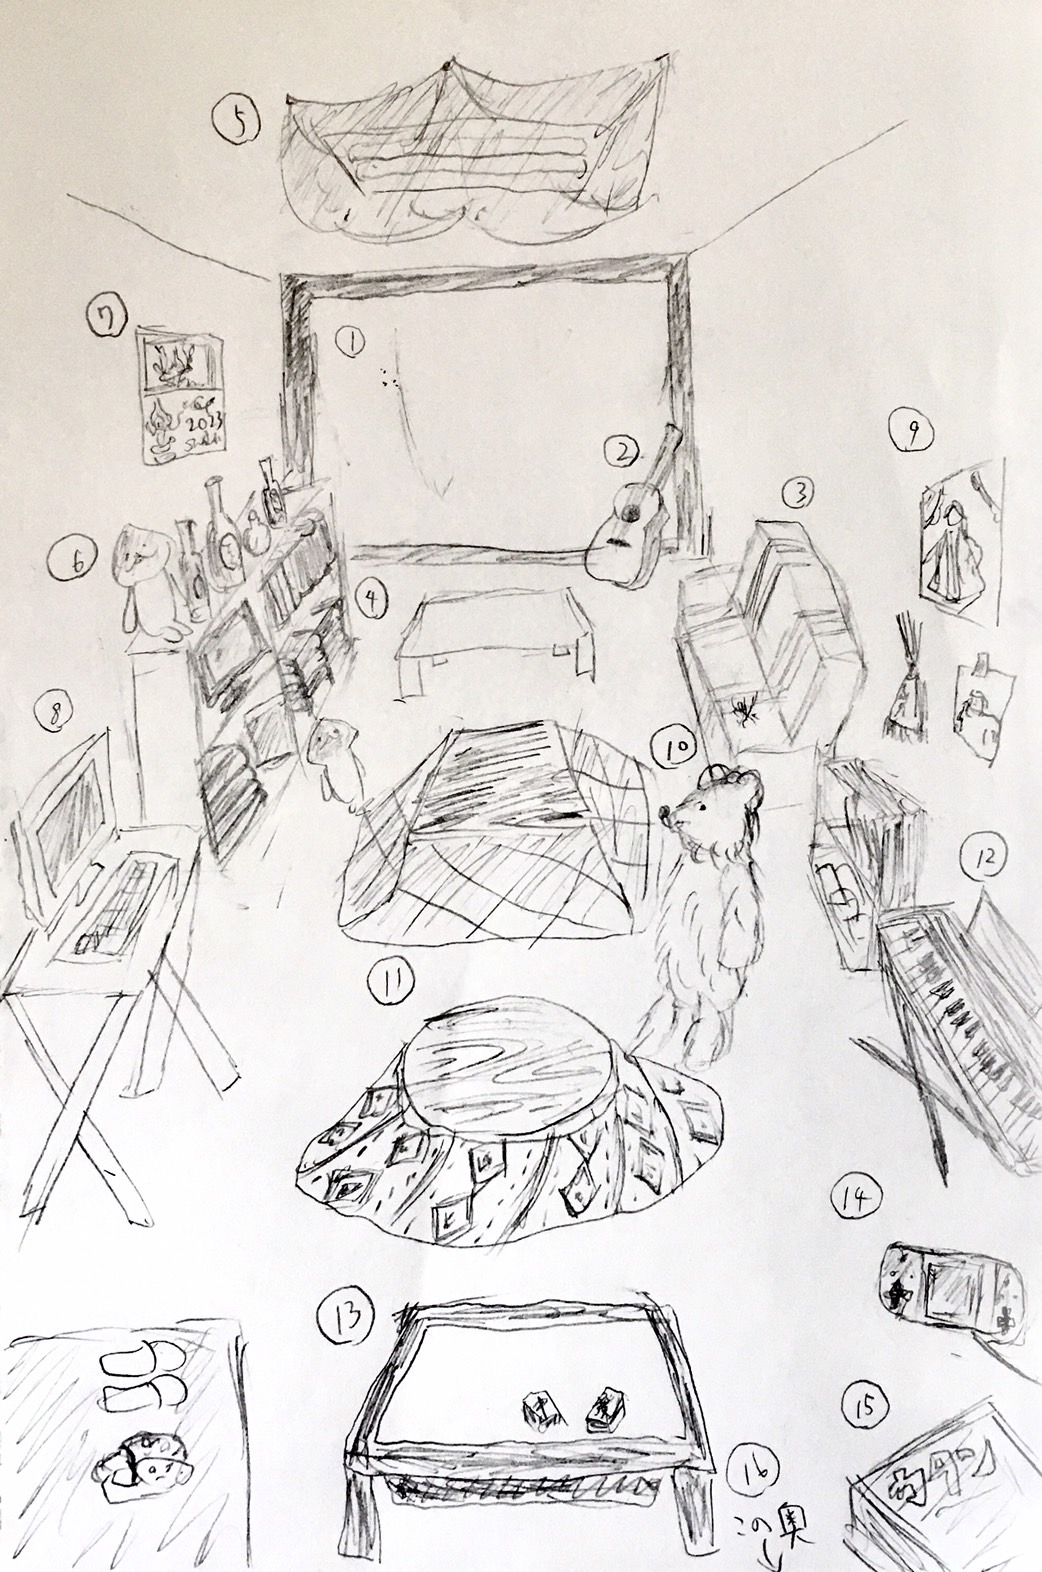
\includegraphics[width=0.59\textwidth]{gazo/C12danwa.jpg}
\end{wrapfigure}

{\small

  \kkkomoku{1}{壁一面のスクリーン}
  C12談話室の一番の特徴。映画ブロックっぽさが出てる。プロジェクターで映してネトフリとかバンドのライブとかの上映会をやっています。

  \kkkomoku{2}{落ちてるギター}
  アコギが落ちています。たまに誰かが練習しているよ。

  \kkkomoku{3}{座るとズボンが破けるソファ}
  なんかちょっと生地が破れてばねが出てるところがあって、そこに座ると立ち上がる時にズボンが破れる。既に複数名の被害者が出ている。

  \kkkomoku{4}{ちょっとだけ漫画の棚}
  C12談話室は他ブロック談話室に比べて漫画が少なめ。でも最近は増えてきていて、今は「乙嫁語り」、「よつばと!」、「宝石の国」、「だもんで豊橋が好きって言っとるじゃん!」などの漫画がある。

  \kkkomoku{5}{暖色の照明+いい感じの布}
  C12の温かい雰囲気を醸し出している。今年度のマイナーチェンジポイント。

  \kkkomoku{6}{大量のなめこのぬいぐるみ}
  誰かの枕になってることも。実は筆者が持ってきた。

  \kkkomoku{7}{インド的カレンダー}
  インド系移民の研究をしている方がお土産に持って帰ってきてくれた。インド感すごい。

  \kkkomoku{8}{共用のパソコン}
  ネトフリとかを使ったり、麻雀の戦績の記録をしたりしているパソコン。

  \kkkomoku{9}{祭壇}
  いろいろなものがごっちゃに祀られている。

  \kkkomoku{10}{巨大なピンクのクマのぬいぐるみ}
  誰かのクッションになりすぎて最近なんかつぶれてきた。

  \hfill

  \hfill
  %位置調節のための改行
  
  \kkkomoku{11}{こたつ}
  談話室の中心、憩いの場、引き寄せられて出られないこたつ。withみかんは最高の冬。5人くらいで入ってることも。最近新しいこたつが増えました!やったー!!!

  \kkkomoku{12}{キーボード}
  他ブロックにはあまりないかも。C12談話室の文化的な面を醸し出す一助となっている。たまに練習してる人がいる。

  \kkkomoku{13}{自動雀卓}
  今年にはいって麻雀が流行り、拾ってきた。ほぼ毎晩大活躍している。赤ドラがちょっと見にくいのが難点。

  \kkkomoku{14}{switchとか}
  他ブロックほどではないがC12談話室にもゲームがある。1年間でさまざまなゲームが流行っては廃れてきた。マリカやりたいなー

  \kkkomoku{15}{カタンとか}
  ボードゲームもあります。結構時間がかかっちゃうものが多いからそんなに頻繁にはできてないけどたまにやると楽しい。

  \kkkomoku{16}{本棚}
  珍しくマンガじゃない本の本棚がある。ハリポタとかレトリック事典とかある。

  }

